% -----------------------------------------------
% Template for SMAC SMC 2013
% adapted and corrected from the template for SMC 2012, which was adapted from that of SMC 2011
% further updated for TENOR 2015, 2016, 2017 and 2018
% -----------------------------------------------

\documentclass{article}
\usepackage{tenor}
\usepackage{ifpdf}
\usepackage[english]{babel}
\usepackage{balance}
\usepackage{listings}


%%%%%%%%%%%%%%%%%%%%%%%% Some useful packages %%%%%%%%%%%%%%%%%%%%%%%%%%%%%%%
%%%%%%%%%%%%%%%%%%%%%%%% See related documentation %%%%%%%%%%%%%%%%%%%%%%%%%%
%\usepackage{amsmath} % popular packages from Am. Math. Soc. Please use the 
%\usepackage{amssymb} % related math environments (split, subequation, cases,
%\usepackage{amsfonts}% multline, etc.)
%\usepackage{bm}      % Bold Math package, defines the command \bf{}
%\usepackage{paralist}% extended list environments
%%subfig.sty is the modern replacement for subfigure.sty. However, subfig.sty 
%%requires and automatically loads caption.sty which overrides class handling 
%%of captions. To prevent this problem, preload caption.sty with caption=false 
%\usepackage[caption=false]{caption}
%\usepackage[font=footnotesize]{subfig}


% REDEFINE THESE VARIABLES:
\def\papertitle{Symbolist: redesigned for dynamic bidirectional mapping}
\def\firstauthor{Rama Gottfried}
\def\secondauthor{James Cheung}
\def\thirdauthor{Georg Hajdu}

\def\copyrightyear{2022}


\usepackage{xspace}
\def\symbolist{\textsc{symbolist}\xspace}
\def\drawsocket{\textsc{drawsocket}\xspace}
\makeatletter
\newcommand{\verbatimfont}[1]{\renewcommand{\verbatim@font}{\ttfamily#1}}
\makeatother


%% Depending on the number of authors, set this variable accordingly for the copyright notice:
% \def\copyrightauthors{Author One}
\def\copyrightauthors{Rama Gottfried, James Cheung and Georg Hajdu}
% \def\copyrightauthors{Author One, Author Two et al}

% adds the automatic
% Saves a lot of output space in PDF... after conversion with the distiller
% Delete if you cannot get PS fonts working on your system.

\def\oscfontsize{\footnotesize}


% pdf-tex settings: detect automatically if run by latex or pdflatex
\newif\ifpdf
\ifx\pdfoutput\relax
\else
   \ifcase\pdfoutput
      \pdffalse
   \else
      \pdftrue
\fi

\ifpdf % compiling with pdflatex
  \usepackage[pdftex,
    pdftitle={\papertitle},
    pdfauthor={\firstauthor},
    bookmarksnumbered, % use section numbers with bookmarks
    pdfstartview=XYZ % start with zoom=100% instead of full screen; 
                     % especially useful if working with a big screen :-)
   ]{hyperref}
  %\pdfcompresslevel=9

  \usepackage[pdftex]{graphicx}
  % declare the path(s) where your graphic files are and their extensions so 
  %you won't have to specify these with every instance of \includegraphics
  \graphicspath{{./figures/}}
  \DeclareGraphicsExtensions{.pdf,.jpeg,.png}

  \usepackage[figure,table]{hypcap}

\else % compiling with latex
  \usepackage[dvips,
    bookmarksnumbered, % use section numbers with bookmarks
    pdfstartview=XYZ % start with zoom=100% instead of full screen
  ]{hyperref}  % hyperrefs are active in the pdf file after conversion

  \usepackage[dvips]{epsfig,graphicx}
  % declare the path(s) where your graphic files are and their extensions so 
  %you won't have to specify these with every instance of \includegraphics
  \graphicspath{{./figures/}}
  \DeclareGraphicsExtensions{.eps}

  \usepackage[figure,table]{hypcap}
\fi

%setup the hyperref package - make the links black without a surrounding frame
\hypersetup{
    colorlinks,%
    citecolor=black,%
    filecolor=black,%
    linkcolor=black,%
    urlcolor=black
}


% Title.
% ------
\title{\papertitle}

% Authors
% Please note that submissions are NOT anonymous, therefore 
% authors' names have to be VISIBLE in your manuscript. 
%
% Single address
% To use with only one author or several with the same address
% ---------------
%\oneauthor
%   {\firstauthor} {Affiliation \\ City, Country \\
%     {\tt \href{mailto:author1@adomain.org}{author1@adomain.org}}}

%Two addresses
%--------------
% \twoauthors
%   {\firstauthor} {Affiliation \\ City, Country \\ 
%     {\tt \href{mailto:author1@adomain.org}{author1@adomain.org}}}
%   {\secondauthor} {Affiliation \\ City, Country \\ 
%     {\tt \href{mailto:author2@adomain.org}{author2@adomain.org}}}

% Three addresses
% --------------
 \threeauthors
   {\firstauthor} { University for Music and Theater \\ Hamburg, Germany \\
     {\tt \href{mailto:rama.gottfried@hfmt-hamburg.de}{rama.gottfried@hfmt-hamburg.de}}}
   {\secondauthor} {University for Music and Theater \\ Hamburg, Germany  \\ 
     {\tt \href{mailto:james.cheung@hfmt-hamburg.de}{james.cheung@hfmt-hamburg.de}}} 
   {\thirdauthor} {University for Music and Theater \\ Hamburg, Germany \\
     {\tt \href{mailto:georg.hajdu@hfmt-hamburg.de}{georg.hajdu@hfmt-hamburg.de}}}


% ***************************************** the document starts here ***************
\begin{document}
%
\capstartfalse
\maketitle
\capstarttrue
%
\begin{abstract}

maybe already start with history here, and then continue to symbolist?

  \symbolist is an in-development application for experimental notation, with the goal of creating a working environment for developing symbolic notation for multimedia which can be interpreted and performed by electronics. The program aims to provide an open play space, with tools for experimentation, and thinking visually about relationships between representation and interpretation in media performance. 
In the paper we discuss the evaluation and re-design of the application based on the need for a bi-directional mapping framework for working with symbolic notation and its corresponding data representations.


\end{abstract}
%

\section{Background}\label{sec:background}


The \symbolist project was developed out of an organic  of compositional notation practice. 

how much of a background?

\quote{
In this paper we present a case study for the creation of an open system for graphically developing symbolic notation which can function both as professional quality print or online documentation, as well as a computer performable score in electro-acoustic music and other computer aided contexts. Leveraging Adobe Illustrator’s graphic design tools and support for the Scalable Vector Graphics (SVG) file format, the study shows that SVG, being based on Extensible Markup Language (XML), can be similarly used as a tree-based container for score information. In the study, OpenSoundControl (OSC) serves as middleware used to interpret the SVG representation and finally realize this interpretation in the intended media context (electronic music, spatial audio, sound art, kinetic art, video, etc.). The paper discusses how this interpretive layer is made possible through the separation of visual representation from the act of rendering, and describes details of the current implementation, and outlines future developments for the project.
}

Initially developed as a method for performing vector graphics, 
SVG-OSC

XML nature of SVG makes it easy to parse and map just like and OSC bundle.

drawing on the OSC research at CNMAT, 

just like a piece of paper, SVG could be freely mappable, and \textit{performable} like OSC.





however it can require a lot of specialized code to handle different hierarchy structures and data at different levels in the hierarchy.


the first version of \symbolist was created as a standalone JUCE application
Ircam/ZKM 

\section{JUCE Version}\label{sec:juce_version}

explain juce version
MVC
focused on creating SVG and outputting OSC version (like SVG-OSC approach)


\section{Clefs and Bidirectional Mapping}\label{sec:bidirectional_mapping}

idea of Clefs

problem:
a lot of mapping is still needed



\section{Symbolist Electron}\label{sec:symbolist_electron}

\begin{figure*}[ht!]
\centering
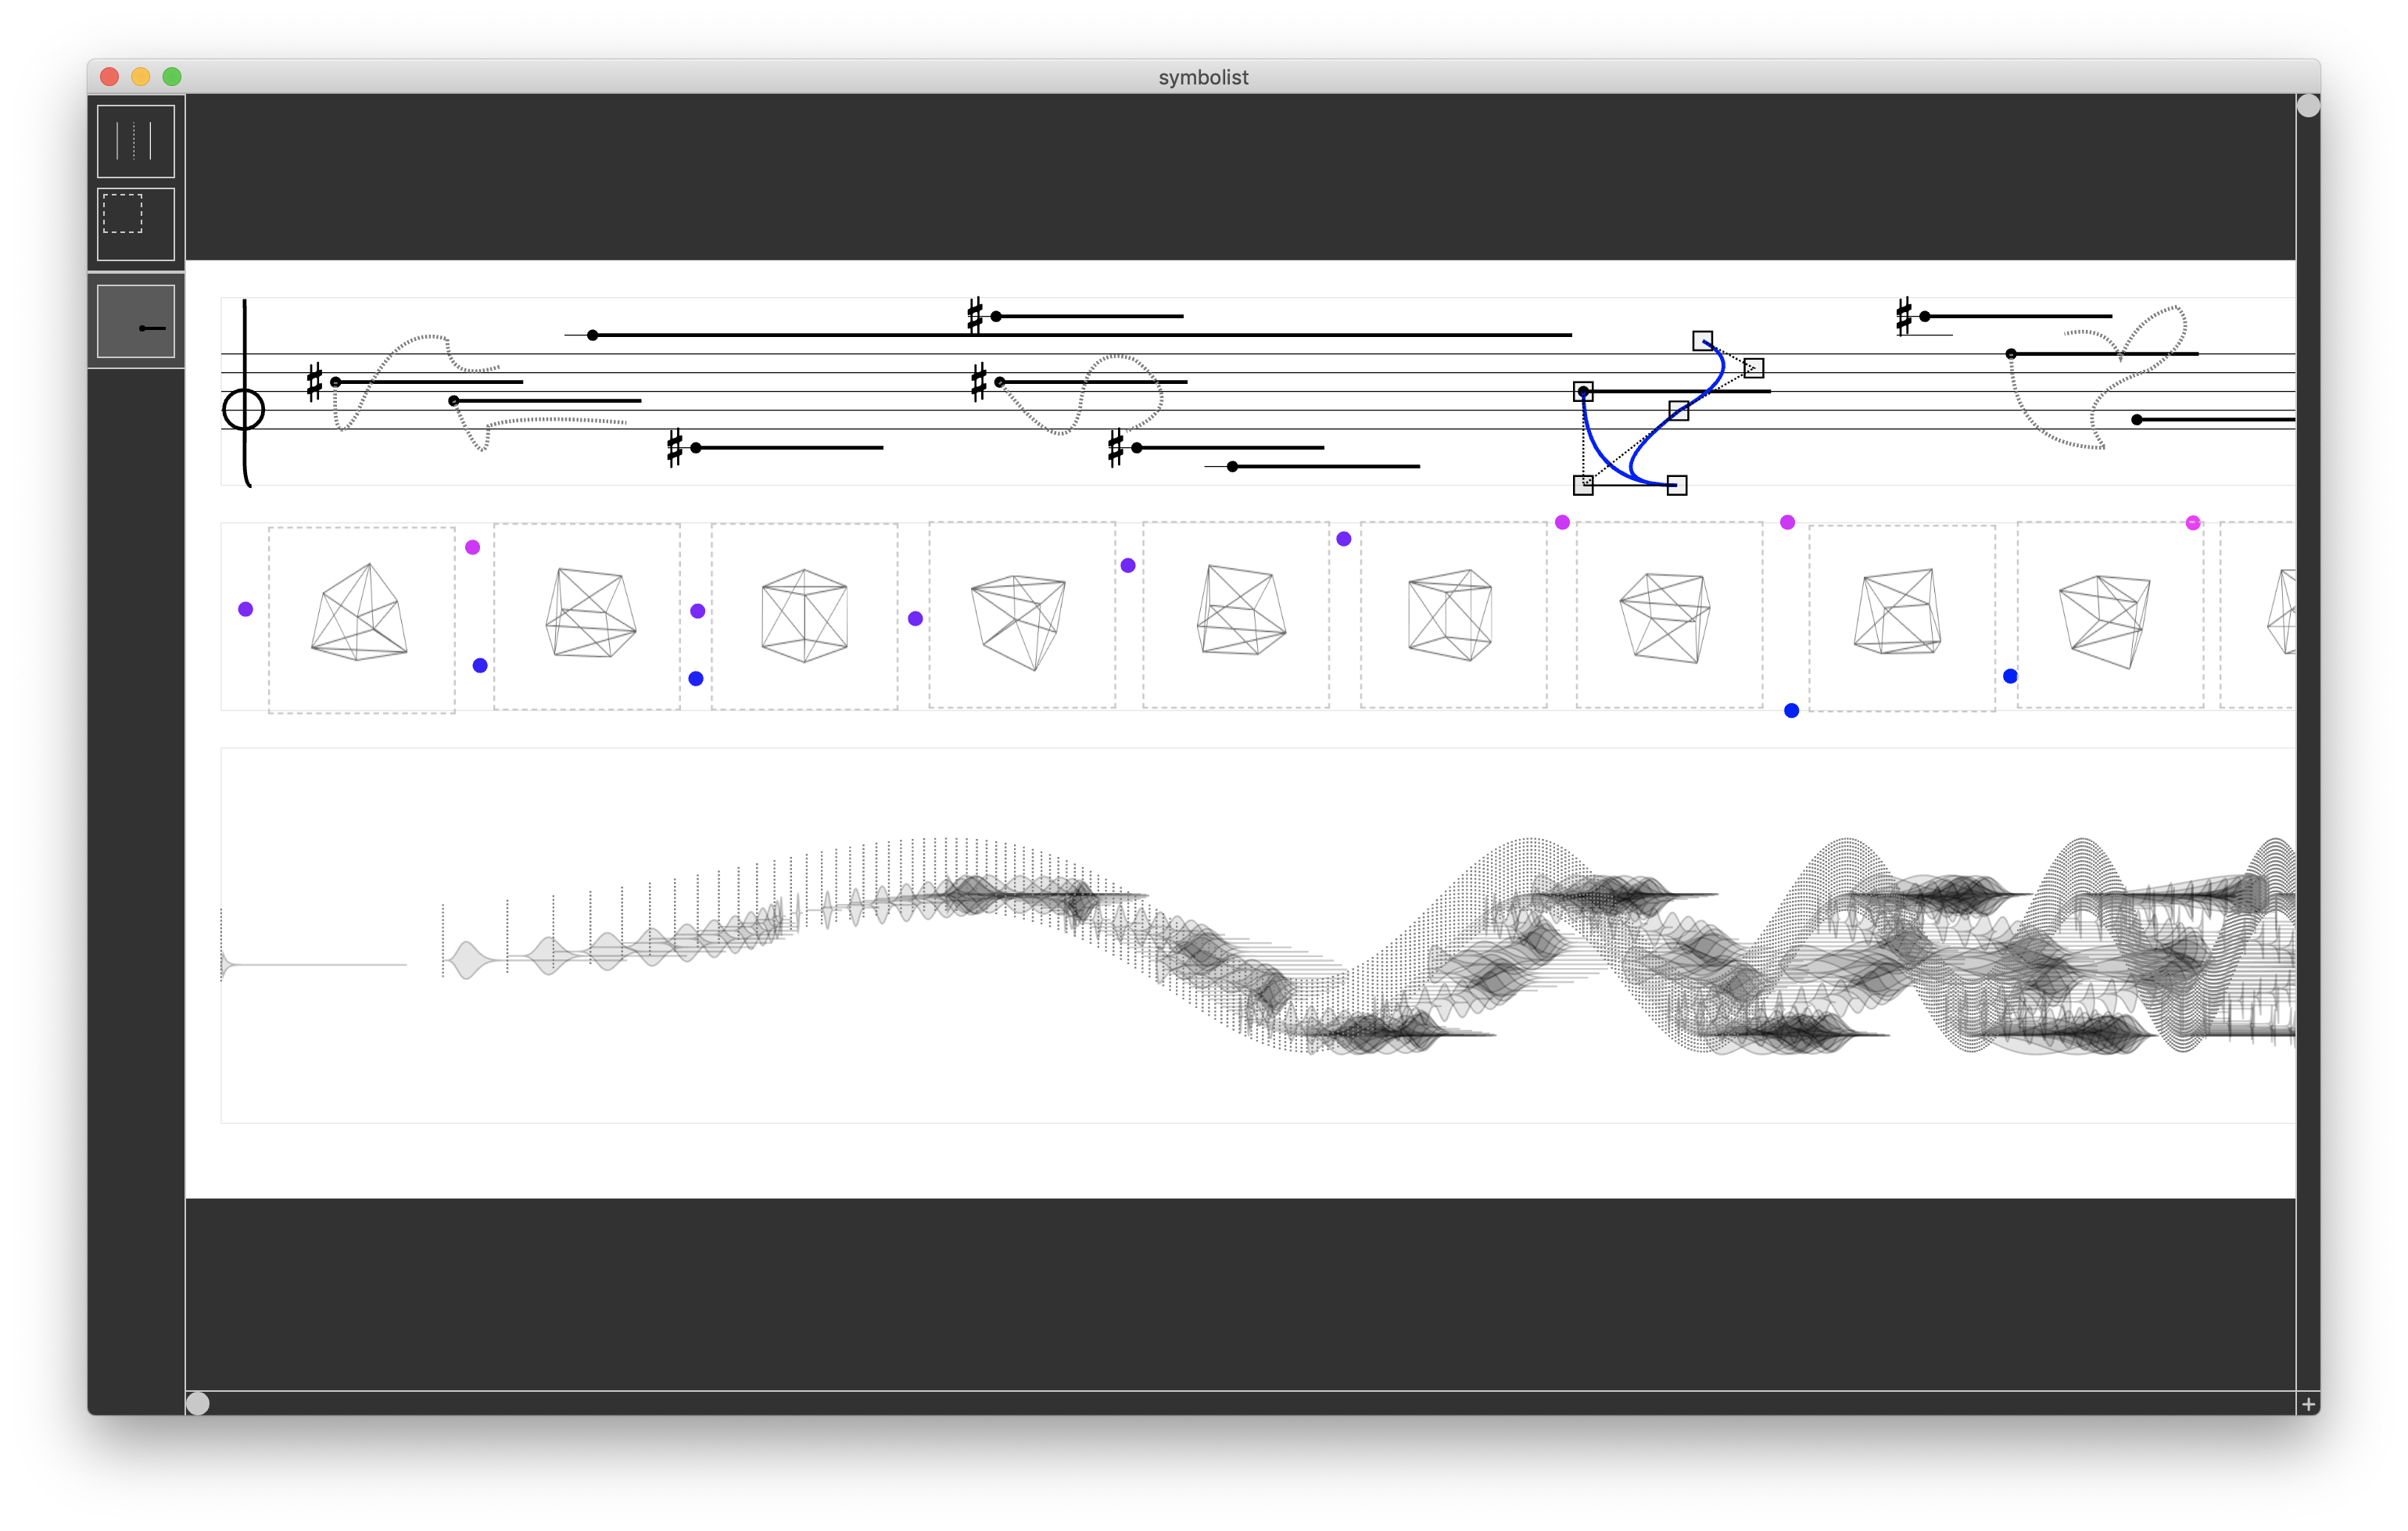
\includegraphics[width=2\columnwidth]{symbolist.png}
\caption{ \symbolist screenshot, showing some different types of staves, and editing capabilities.
\label{fig:screenshot}}
\end{figure*}


a general overview about need for classes, js and \drawsocket makes that easy(-ier)
using \drawsocket as front end handler

Figure~\ref{fig:screenshot} shows a screenshot from the Electron version.



\subsection{Max}\label{sec:Max}

Electron version (node + chrome w/ special electron IPC)
Max version (node + jweb + Max patch for IPC)

\subsection{Contexts}\label{subsec:contexts}

There are three basic representation contexts at the core of \symbolist:

\begin{enumerate}\itemsep0pt
\item \textbf{semantic data}, which specifies the various attributes of information about a symbolic object, in terms of the \textit{meaning} to the author. The  \textit{semantic data} is the main holder of information in the system, which arranged as a score can function like a database of hierarchal information. For example, a note might contain information about pitch and duration, or a point in space might contain x, y, and z values.
\item \textbf{graphic representation}, the visual representation of the semantic data (see figure~\ref{fig:graphic-representation}).
\item \textbf{performance media}, the performance mechanism which can be used to control different media types using the score data as parameter values. 
\end{enumerate}



\begin{figure}[ht!]
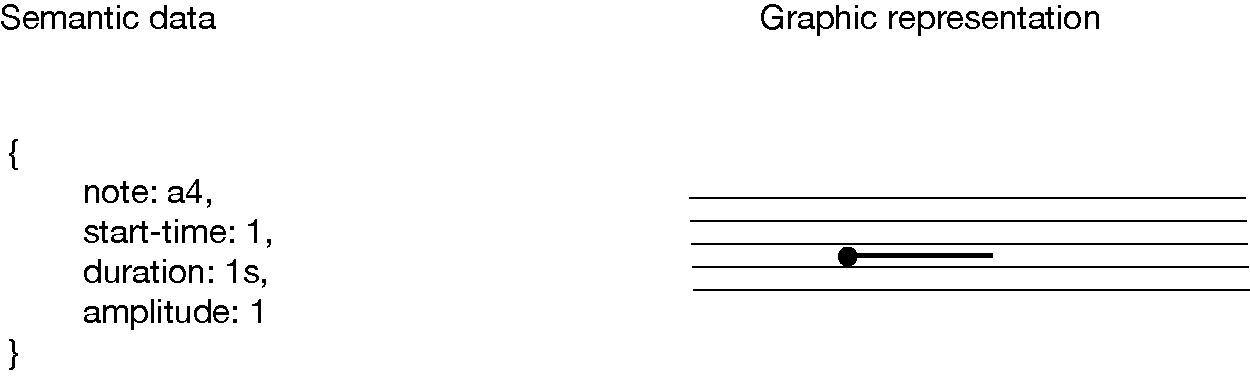
\includegraphics[width=1\columnwidth]{graphic-representation.pdf}
\caption{\textit{data} vs \textit{graphic} representation of the same information.
\label{fig:graphic-representation}}
\end{figure}



\subsection{Mapping}\label{subsec:mapping}

Between each of these representation contexts there is a layer of mapping:

\begin{itemize}\itemsep0pt % use \itemsep if necessary to reduce space between items
\item \textit{semantic data} to \textit{graphic representation} is used for the creation of graphic symbols based on input of semantic data.
\item \textit{graphic representation} to \textit{semantic data} is used to edit, or create new data entries, based on graphic information.
\item \textit{semantic data} to \textit{performance media} is the use of the data as a sequence of events that can be played in time (or used to control other processes not necessarily in time).
\item mapping between \textit{performance media} and \textit{graphic representation} is achieved through first mapping to semantic data.
\end{itemize}

\begin{figure}[ht!]
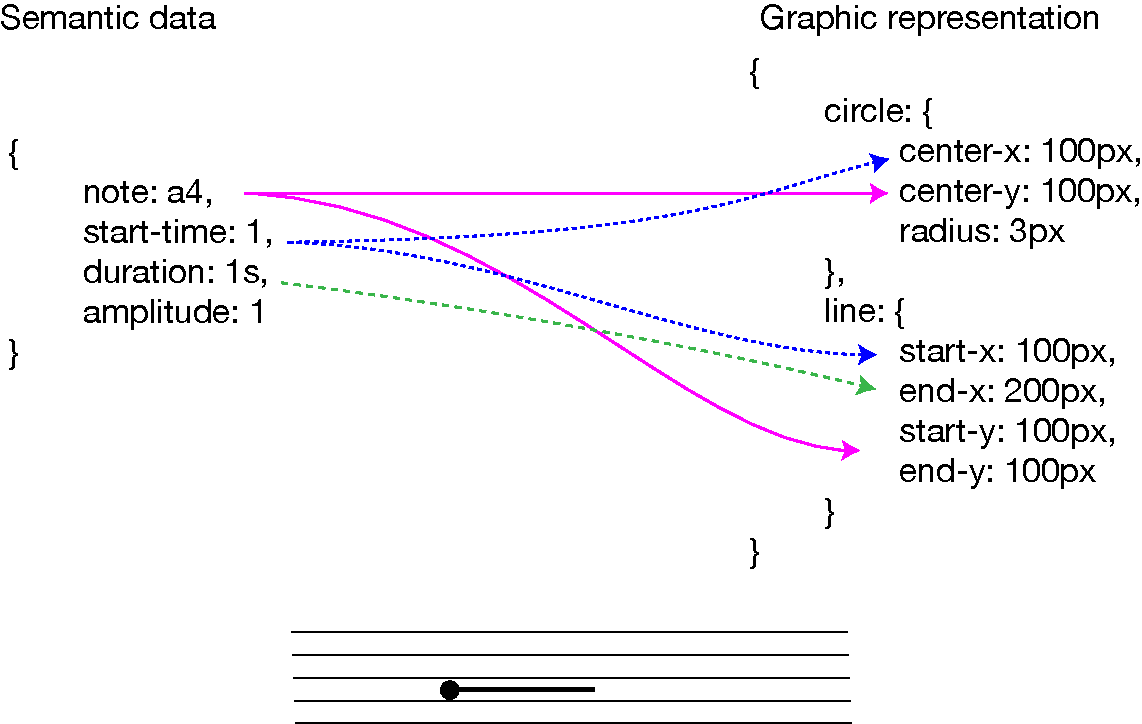
\includegraphics[width=1\columnwidth]{data-to-graphic.pdf}
\caption{\textit{semantic data} mapped to create a \textit{graphic} representation from input data.
\label{fig:data-to-graphic}}
\end{figure}


\begin{figure}[ht!]
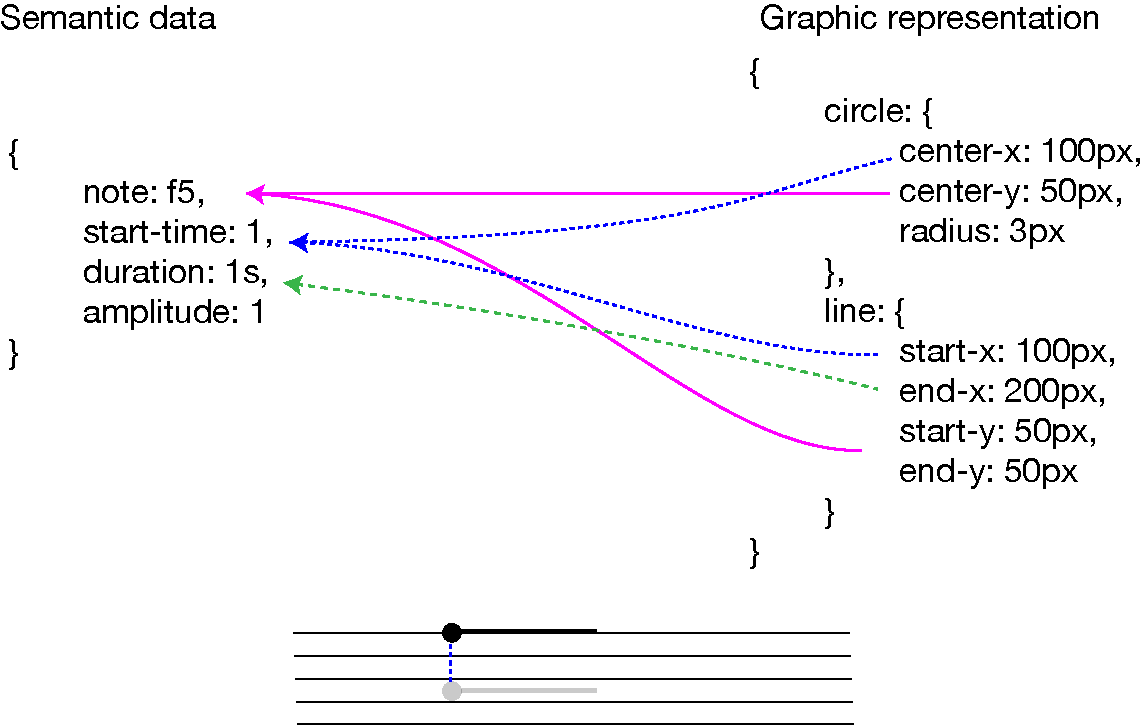
\includegraphics[width=1\columnwidth]{graphic-to-data.pdf}
\caption{If edited graphically, the updated graphic data is then mapped back to \textit{semantic data} representation. 
\label{fig:graphic-to-data}}
\end{figure}


\begin{figure}[ht!]
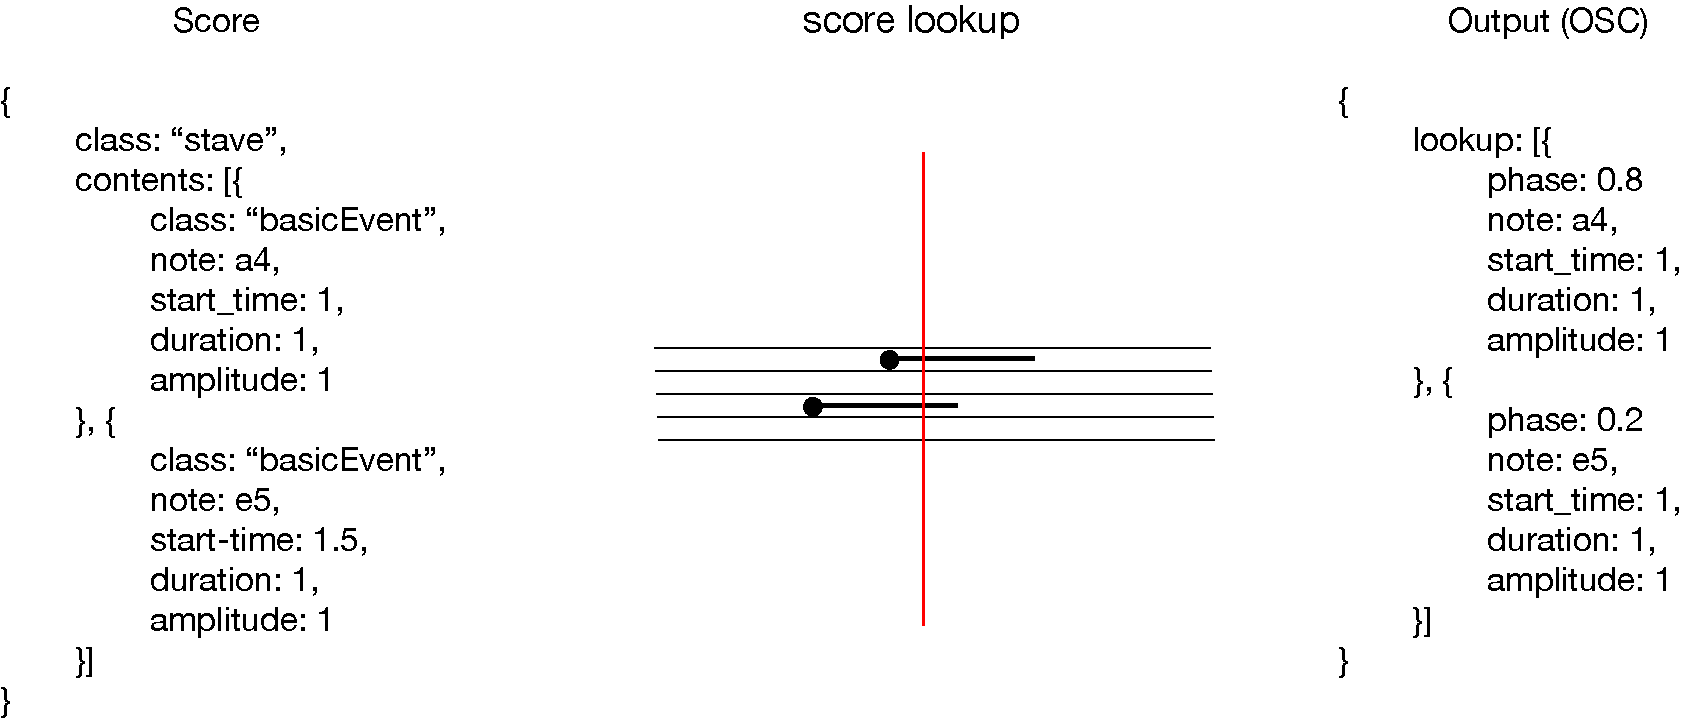
\includegraphics[width=1\columnwidth]{score-lookup.pdf}
\caption{Using the lookup method defined by the symbol class, the \textit{semantic data} can be used to perform external instruments via Open Sound Control. 
\label{fig:score-lookup}}
\end{figure}


\subsection{Application Structure}\label{subsec:application_structure}

The main structure of the platform is currently in three parts:

\begin{enumerate}\itemsep0pt
\item The \textit{editor}, a browser-based graphic user interface which displays the graphic representation of the data, and allows the user to edit and create new data from graphic interaction. The editor loads a library of scripts that define mappings to and from data and graphics formats. The editor receives and outputs data in the semantic format, keeping the concerns of drawing within the browser-side.

\item The \textit{server}, a node.js (or electron) based webserver which routes messages between the \textit{editor} and the \textit{io} system, and handles operating system commands like reading and writing files.

\item  The \textit{io-server}, which handles input and output from external sources via OSC. The \textit{io-server} holds a copy of the score in its semantic format, and loads a parallel library of user scripts to the \textit{editor} which define the mapping to (and potentially from) other media sources. The \textit{io-server} might also be used to reformat the score into a format that can be performed by another sequencing tool or program like MaxMSP.
\end{enumerate}

\begin{figure*}[ht!]
\centering
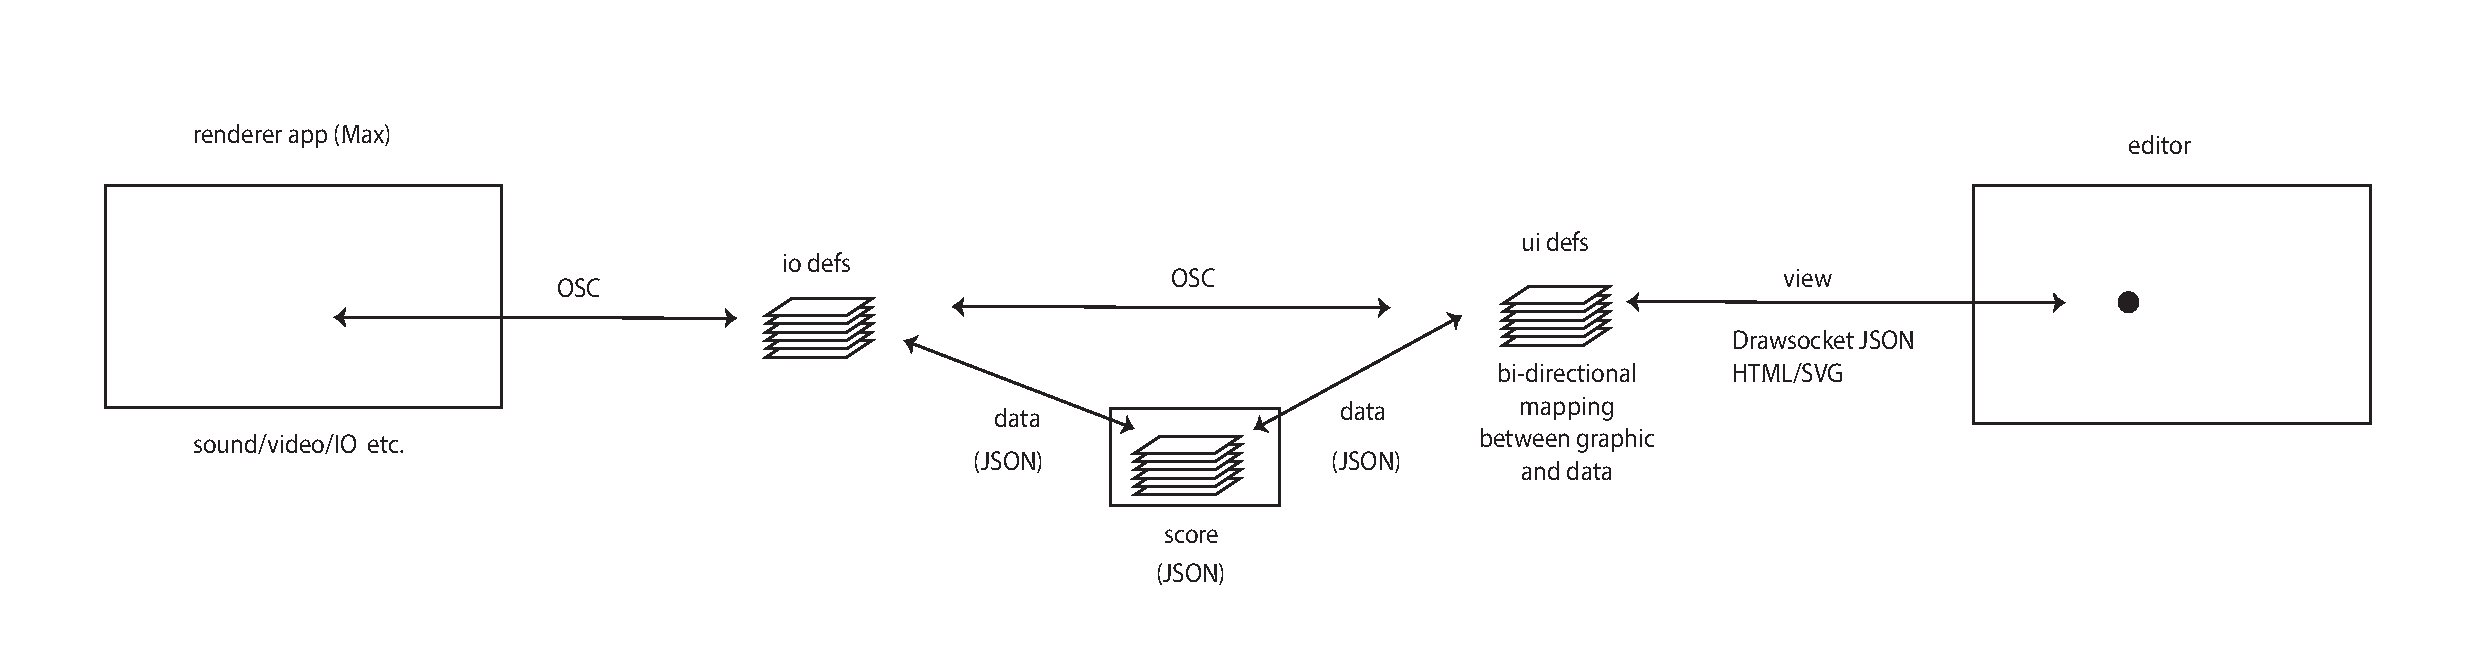
\includegraphics[width=2\columnwidth]{symbolist-architecture.pdf}
\caption{ \symbolist architecture.
\label{fig:architecture}}
\end{figure*}


\subsubsection{io and ui elements}\label{subsec:io_ui_elements}

discuss using DOM elements for hierarchy and document.querySelector in ui
and similar options in io using score vs model




\subsection{Symbols}\label{subsec:symbols}

The \textit{semantic data} is stored in a \textit{model} or \textit{score} which is made up of a hierarchical arrangement of objects called \textit{symbols}.

Each \textit{symbol} is a data object which holds a set of data parameters. For example a typical event like \textit{symbol} might represent a note event, and contain \textit{pitch},  \textit{time} and \textit{duration} parameters. The details of each symbol's data structure and UI interaction is defined in an object \textit{class}.

CHECK IF CONTAINERS STILL EXIST, edit that out probably
everything can be a container
IN SCORE, CONTAINER IS USED TO IDENTIFY PARENT ELEMENT (but it's not a class)


\textit{symbols} may also be containers that contain other symbols. Container symbols function to frame their contents, giving them reference and context, like a plot graph frame, which provides a perspective for interpreting a set of data points.

In most cases, a symbol mapping definition will require querying the parent container symbol for information, to plot the data into the container frame's context. 

All symbols are stored in container symbols.
\subsection{JSON}\label{subsec:json}

Data is stored in JSON format.

The main object data attributes are:
\begin{itemize}\itemsep0pt % use \itemsep if necessary to reduce space between items
\item \textit{id}: a unique identifier name.
\item \textit{class}: a reference to the definition of the object type in the user-definition library.
\item \textit{contents}: an array of other objects that a container object holds.
\end{itemize}

For example a simple \textit{symbol} object might look like:


\begin{lstlisting}[
  mathescape,
  columns=fullflexible,
  breaklines=true,
  basicstyle=\oscfontsize\fontfamily{lmvtt}\selectfont,
]
{
    "id" : "foo",
    "class" : "legs",
    "action" : "jump",
    "startTime" : 0.1
}
\end{lstlisting}

Here we see an object with the \textit{id} ``foo,'' which is of class type \textit{legs}, that has an attribute \textit{action} associated with it and a start time.

And here is a simple example of a \textit{container} object of a type class \textit{timeline}, which holds two types of leg actions:

\begin{lstlisting}[
  mathescape,
  columns=fullflexible,
  breaklines=true,
  basicstyle=\oscfontsize\fontfamily{lmvtt}\selectfont,
]
{
    "id" : "bar",
    "class" : "timeline",
    "duration" : 1,
    "contents" : [{
        "id" : "foo-1",
        "class" : "legs",
        "action" : "jump",
        "startTime" : 0.1
    },{
        "id" : "foo-2",
        "class" : "legs",
        "action" : "sit",
        "startTime" : 0.2
    }]
}

\end{lstlisting}

\subsection{File Format}\label{subsec:file_format}

Symbolist files are composed in the same way that the data model is stored. The top level symbol will be created in the `top-svg` symbol which is pre-defined in the `index.html` file.

An example initialization config file might look like this:

\begin{lstlisting}[
  mathescape,
  columns=fullflexible,
  breaklines=true,
  basicstyle=\oscfontsize\fontfamily{lmvtt}\selectfont,
]
{
    "about" : "symbolist will read a json file to configure the palette setup, this can be used to dynamically change the application layout and tools",
    "id" : "Score",
    "tools" : [],
    "palette" : ["SubdivisionTool", "BasicSymbolGL"],
    "class" : "RootSymbol",
    "contents": { 
        "id" : "trio",
        "class" : "SystemContainer",
        "x": 200,
        "y": 100,
        "duration": 20,
        "time": 0,
        "contents" : [{
            "id" : "oboe",
            "class" : "FiveLineStave",
            "height" : 100,
            "lineSpacing" : 10,
            "duration": 20,
            "time": 0,
            "contents" : []
        },
        {
            "id" : "bassoon",
            "class" : "PartStave",
            "height" : 100,
            "time": 0,
            "duration": 20,
            "contents" : []
        },
        {
            "id" : "synth",
            "class" : "PartStave",
            "height" : 200,
            "time": 0,
            "duration": 20,
            "contents" : []
        }]
    }
}
\end{lstlisting}


\subsection{Graphic Display Format}\label{subsec:file_format}

The graphic representation of symbols is in SVG format, which is laid out in the `index.html` file. The \drawsocket SVG/HTML/CSS wrapper is being used for convenience, to provide a shorthand method of creating and manipulating browser window elements. However, since the \textit{ui\_controller} and user definition scripts are all being processed in the browser, scripts are free to use traditional JS approaches to manipulating the browser DOM.

Since `symbolist` is constantly mapping to and from semantic data and its graphic representation, we are using the HTML \textit{dataset} feature to store the semantic data inside the SVG object.

Typically, the `id` attribute is used to quickly identify graphic objects, for the sake of clarity this is being left out of the examples below.

\subsection{Symbol}\label{subsec:symbol}

\begin{minipage}{\linewidth}
The SVG \symbolist format for a \textit{symbol} is a one top group ($<$g$>$) elements, with two sub-groups:

\begin{lstlisting}[
  mathescape,
  columns=fullflexible,
    breaklines=true,
  basicstyle=\oscfontsize\fontfamily{lmvtt}\selectfont,
]
<g  class="symbolClassName symbol" data-time="0.1" data-duration="1">
    <g class='symbolClassName display'></g>
    <g class='symbolClassName contents'></g>
</g>
\end{lstlisting}
\end{minipage}



Each symbol grouping element is tagged using CSS class names, following the symbol's unique class name (in this example ``symbolClassName''):
\begin{itemize}\itemsep0pt 
\item \textit{symbol} marks the top-level grouping object of the symbol
\begin{itemize}\itemsep0pt 
  \item \textit{display} a group that holds the visual display of the container symbol, and
  \item \textit{contents} which contains other symbols.
  \end{itemize}
\end{itemize}



Note that the order is important: \textit{the symbol class type must be first}.

The semantic data is also stored in the top-level symbol $<$g$>$ element, using the HTML dataset feature, marked with the prefix `data-`.

For example:

\begin{lstlisting}[
  mathescape,
  columns=fullflexible,
    breaklines=true,
  basicstyle=\oscfontsize\fontfamily{lmvtt}\selectfont,
]
<g  class='containerClassName symbol container' data-time='0.1' data-duration='1'>
    <g class='containerClassName display'>
         <line .... />
    </g>
    <g class='containerClassName contents'>
        <g class"symbolClassName symbol" data-time="0.1" data-duration="1">
            <circle .... />
        </g>
    </g>
</g>
\end{lstlisting}


Symbols and containers could also potentially be HTML elements instead of SVG. In the case of HTML you would use $<$div$>$ tags instead of SVG $<$g$>$:
html:

\begin{lstlisting}[
  mathescape,
  columns=fullflexible,
  basicstyle=\oscfontsize\fontfamily{lmvtt}\selectfont,
]
<div class='containerClassName symbol container'>
    <div class='containerClassName display'></div>
    <div class='containerClassName contents'></div>
</div>
\end{lstlisting}




\subsection{IO Messages}\label{subsec:io_messages}

\symbolist has built in handlers for a set of messages received via OSC, which can be extended by user scripts, using a key/val syntax, where the \textit{key} specifies the function to call, and the \textit{val} are the parameter values to use for the call.

For example, here is a \textit{lookup} query to find elements that are returned by the parameters \textit{time} in the container with the \textit{id} ``trio''.


\begin{lstlisting}[
  mathescape,
  columns=fullflexible,
  basicstyle=\oscfontsize\fontfamily{lmvtt}\selectfont,
]
{
    /key : "lookup:,
    /val : {
        /time : 0.1,
        /id : "trio"
    }
}

\end{lstlisting}

The OSC message API supports the following keys:
\begin{itemize}\itemsep0pt 
\item \textit{data}: adds a data object to the score, and sends to the ui to be mapped to graphical representation. Parameters include:
\begin{itemize}\itemsep0pt 
  \item \textit{class} (required) the class type of the object to create
  \item \textit{container} (required) the container symbol class to put the object in (in case there are multiple containers that support the same symbol type)
  \item \textit{id} (optional) an id to use for the data object, if non is specified a (long) unique string will be generated.
  \item Other required or optional parameters will depend on the symbol definition.
\end{itemize}

\begin{lstlisting}[
  mathescape,
  columns=fullflexible,
  basicstyle=\oscfontsize\fontfamily{lmvtt}\selectfont,
]
{
    /key : "data",
    /val : {
        /class : "fiveLineStaveEvent",
        /id : "foo"
        /container : "oboe",
	    /time : 0.13622,
	    /ratio : "7/4",
	    /duration : 0.1,
	    /amp : 1
    }
  }
\end{lstlisting}


\item \textit{lookup}: looks up a point in a container, based on a sorting function specified in the definition. For example, this can be used to get all events active at a given time. Parameters:

\begin{itemize}\itemsep0pt 
  \item \textit{id}: (required) the \textit{id} of the container to lookup in. Containers will generally iterate all child objects, so for example if you use the \textit{id} of the top level score you should be looking up in to all sub-containers.
  \end{itemize}
  
\item \textit{getFormattedLookup}: optional function that might be defined in an \textit{io} script that outputs an object formatted for a different type of player/render. For example, this function might return a list of \textit{/x} and \textit{/y} values for use with the \textit{o.lookup~} Max object, or create a MIDI file export etc. All parameters included in the \textit{val} object will be sent to the \textit{getFormattedLookup} as a parameters object. Parameters:

\begin{itemize}\itemsep0pt 
  \item \textit{id}: (required)
\end{itemize}
\item \textit{call}: calls a function in the one or both of the class definitions. All of the parameters in the \textit{val} object will be passed to the function as an argument. Return values from the \textit{io} controller are with the tag \textit{return/io} and \textit{return/ui} from the \textit{ui}.
\begin{itemize}\itemsep0pt 
  \item \textit{class} (required) class of the object to call
  \item \textit{method} (required) name of object function to call
\end{itemize}

\end{itemize}

\begin{lstlisting}[
  mathescape,
  columns=fullflexible,
  basicstyle=\oscfontsize\fontfamily{lmvtt}\selectfont,
]
{
    /key : "call",
    /val : {
        /function : "functionName",
        /class : "className",
        /id : "foo"
        /someValue : 1,
        /anotherValue : 2
    }
}
\end{lstlisting}

Note that the system will pass the same call to both definitions, so if both have a function of the same name they will both be called.
* \textit{drawsocket}: forwards \drawsocket format messages directly to \drawsocket, bypassing the symbolist mapping.


\subsection{Library Definitions API}\label{subsec:library_definitions_api}

MENTION CALL METHOD SYSTEM	


discuss BaseClass system


Definition scripts are composed as Javascript modules which are loaded into the program at runtime.

Eventually it is planned to provide a set of tools in the GUI for defining a mapping definition graphically but this is not yet implemented.

There are two types of definition scripts:
* `ui` definitions perform user interactions and mapping between semantic data representation and graphic representation.
* `io` definitions are used to assist in the lookup/playback and mapping of the semantic data to media like sound synthesis, video, etc.

Currently, the system uses the same `.js` file to hold both the `ui` and `io` definitions. To aid in development there is a template file that can be used to handle most of the most common actions.

Using the template, a basic definition might look like this:

%
%
%\begin{lstlisting}[
%  mathescape,
%  columns=fullflexible,
%  basicstyle=\oscfontsize\fontfamily{lmvtt}\selectfont,
%]
%const Template = require('../lib/SymbolTemplate') 
%
%class BasicSymbol extends Template.SymbolBase 
%{
%    constructor() {
%        super();
%        this.class = "BasicSymbol";
%    }
%
%
%    get structs () {
%        return {
%
%            data: {
%                class: this.class,
%                id : `\${this.class}-0`,
%                time: 0,
%                pitch: 55,
%                duration: 0.1
%            },
%            
%            view: {
%                class: this.class,
%                id: `\${this.class}-0`, 
%                x: 0,
%                y: 0,
%                r: 2
%            }
%        }
%    }
%
%
%    display(params) {
%
%        ui_api.hasParam(params, Object.keys(this.structs.view) );
%        
%        return {
%            new: "circle",
%            class: 'notehead',
%            id: `\${params.id}-notehead`,
%            cx: params.x,
%            cy: params.y,
%            r: params.r
%        }
%    }
%    
%    getElementViewParams(element) {
%
%        const circle = element.querySelector('.notehead');
%        const x = parseFloat(circle.getAttribute('cx'));
%        const y = parseFloat(circle.getAttribute('cy'));
%        const r = parseFloat(circle.getAttribute('r'));
%
%        return {
%            id: element.id,
%            x,
%            y,
%            r
%        }
%
%    }
%
%
%    getPaletteIcon() {
%        return {
%            key: "svg",
%            val: this.display({
%                id: `circle-palette-icon`,
%                class: this.class,
%                x: 10,
%                y: 10,
%                r: 2
%            })
%        }
%    }
%
%
%}
%
%class BasicSymbol_IO extends Template.IO_SymbolBase
%{
%    constructor()
%    {
%        super();
%        this.class = "BasicSymbol";
%    }
%    
%}
%
%module.exports = {
%    ui_def: BasicSymbol,
%    io_def: BasicSymbol_IO    
%}
%\end{lstlisting}
%




\subsection{Editor}\label{subsec:editor}

The graphic user interface of \textit{symbolist} is designed around the idea of symbol objects and containers. Graphic objects, or \textit{symbols} are placed in \textit{container} references which define a framing used to interpret the meaning of the \textit{symbol}.

In order to maintain an open and un-opinionated approach to authoring tools, \symbolist tries not to specify how containers and symbols should look, act, or respond when you interact with them within the application. Rather, the interaction and meanings of the symbols are defined in a library of object \textit{definitions} which create these meanings through mapping semantic data to and from the graphic visualization. Definitions can be shared and loaded to setup different composition environments.

See below for more information about the API for creating symbol definitions. 

\subsubsection{Interface Components}\label{subsec:interface_components}

The \symbolist graphic editor provides a set of basic tools for creating scores using the defined symbols and containers:
\begin{itemize}\itemsep0pt % use \itemsep if necessary to reduce space between items
\item \textit{document view}: the top level view of the application window.
\item \textit{menu bar}: the menu bar at the top of the screen or window, which provides access to various application functions.
\item \textit{palette}: a set of buttons on in the side bar of the program which display icons of the `symbols` that have been defined for the current selected \textit{container}. 
\item \textit{tools}: (not yet implemented in the current version) a set of interactive tools that provide ways of creating new symbols, and applying transformations to existing elements (e.g. alignment of multiple objects, or setting distributing objects, etc.)
\item \textit{inspector}: a contextual menu for editing the semantic data of an object, which is then mapped to the graphic representation.
\end{itemize}

On entering the application, the editor loads a score or initialization file from the default load folder, or you can load a new config file after loading. The config file sets the top-level page setup and palette options.

A typical sequence of creating a score might be as follows:
\begin{enumerate}\itemsep0pt
\item the user opens a workspace, with one or more containers displayed on the screen, for example an empty rectangle which is like a piece of paper.
\item selecting the "paper" container rectangle, the user then sets the container as the new `context`, by pressing the `[s]` key (or selecting from the application menu).
\item once setting the context, the `palette` toolbar is populated with icons of symbols that are defined with the selected container context type.
\item clicking on one of the symbol icons, puts the interface into "creation" or "palette mode", where the mouse interaction is now designed for use with this specific symbol type.
\item holding the CMD button, creates a preview of the symbol how it will appear when you click, and some text is displayed near the mouse that shows the semantic data associated with the graphic representation.
\item after clicking the symbol is placed in the container.
\item depending on the symbol type, you may be able to drag the symbol to a new place in the container, and the associated data is updated as a result.
\item selecting the symbol and hitting the `[i]` button, brings up the inspector window, where you can edit the data and see the graphics updated in response.
\item selecting and pressing the `[e]` button enters "edit mode" which is a modal context where different user interaction could change the values of the symbol in different ways. For example in edit mode you might be able to rotate an object in a certain way, or be able to visualize different connections to the graphic representation to other elements of the score which are not usually highlighted in the score view.
\end{enumerate}





\section{NodeScore}\label{sec:node_score}



\section{Floats and equations}

\begin{figure*}[ht!]
\centering
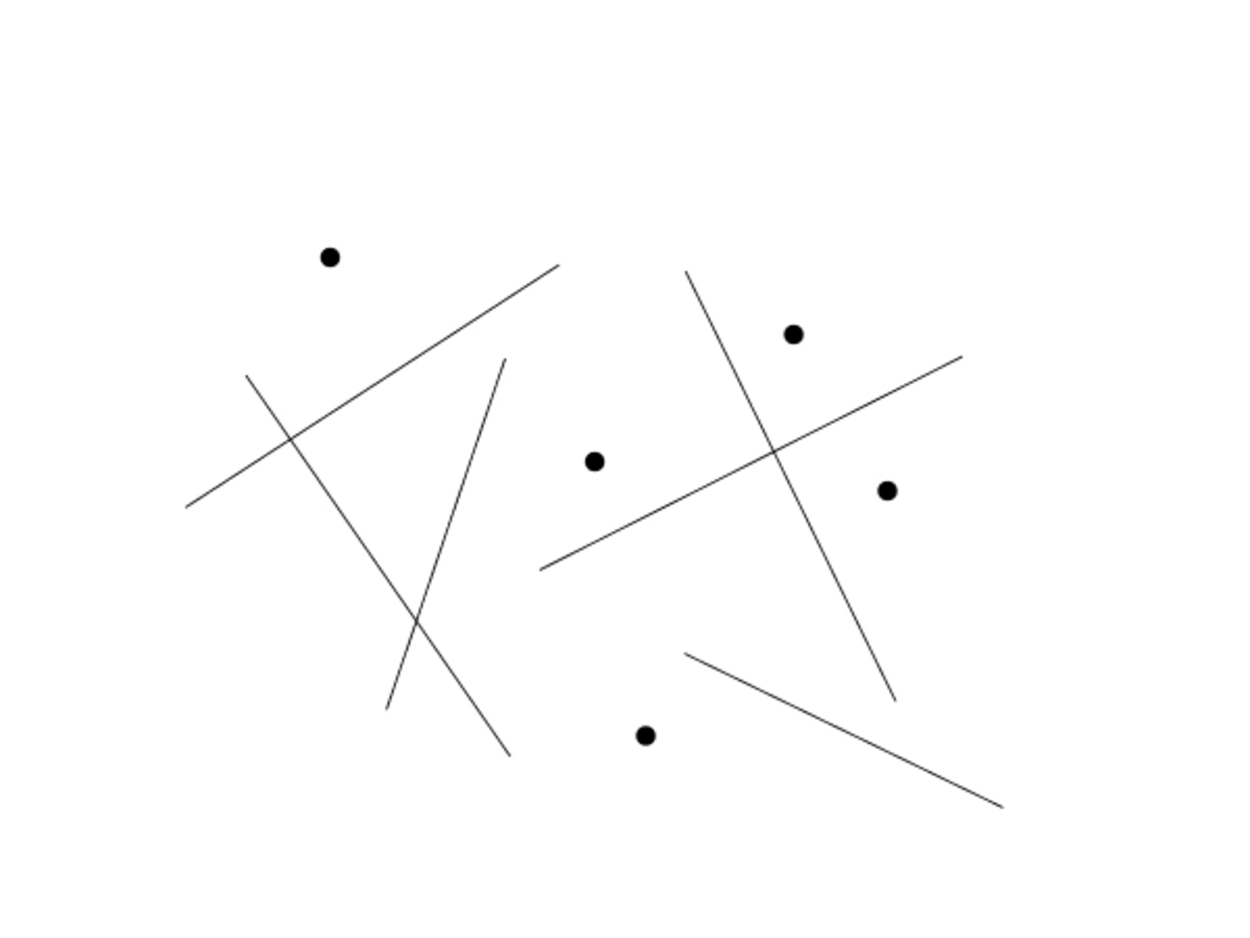
\includegraphics[width=1.5\columnwidth]{figure}
\caption{Using \texttt{figure*}, the figure spans two columns. Captions should be placed below the figure, exactly like this.
\label{fig:example}}
\end{figure*}


\subsection{Figures, Tables and Captions}

\begin{table}[ht!]  % recommented placement insctructiosn for table
\centering 
\begin{tabular}{|l|l|}
  \hline
  String value & Numeric value \\
  \hline
  Hello TENOR  & 2019 \\
  \hline
 \end{tabular}
 \caption{Table captions placed below the table.}
 \label{tab:example}
\end{table}

All artwork must be centered, neat, clean, and legible. 
All lines should be very dark for purposes of reproduction and artwork should not be hand-drawn. The proceedings will be distributed in electronic form only, therefore color figures are allowed.
However, you may want to check that your figures are understandable even if they are printed in black-and-white. 
Vectorial figures are preferred. 
In order to optimize readability, the font size of text within a figure should be at least identical to footnote font size (8pt). 
If bitmap figures are used, please make sure that the resolution is enough for print quality. 

Figure and tables are numbered consecutively. Place tables/figures in text as close to the reference as possible, and preferably at the top of the page. Inline insertion of figures is preferred. Beware of the overall text and columns formatting when placing figures, in order to avoid blank space at the bottom of columns. 
Figures and tables may extend across both columns to a maximum width of 17.2cm.

Numbers and captions of figures and tables always ap-pear below the figure/table. Figure and table captions must follow the model below, with 10pt Times font, bold face for figure/table label and number, and a small spat of 3pt before and after. Captions must be justified on the whole column width if composed of several lines, of centered in case of a single line. 
In principle \LaTeX{} will deal with most of these issues for you.

\textbf{All figures and tables must be referred to in the main text body}, for example: see Figure~\ref{fig:example} and Table~\ref{fig:example} (not Fig.~\ref{fig:example}, or figure~\ref{fig:example}). 


%\begin{figure}[t]
%\figbox{
%\subfloat[][]{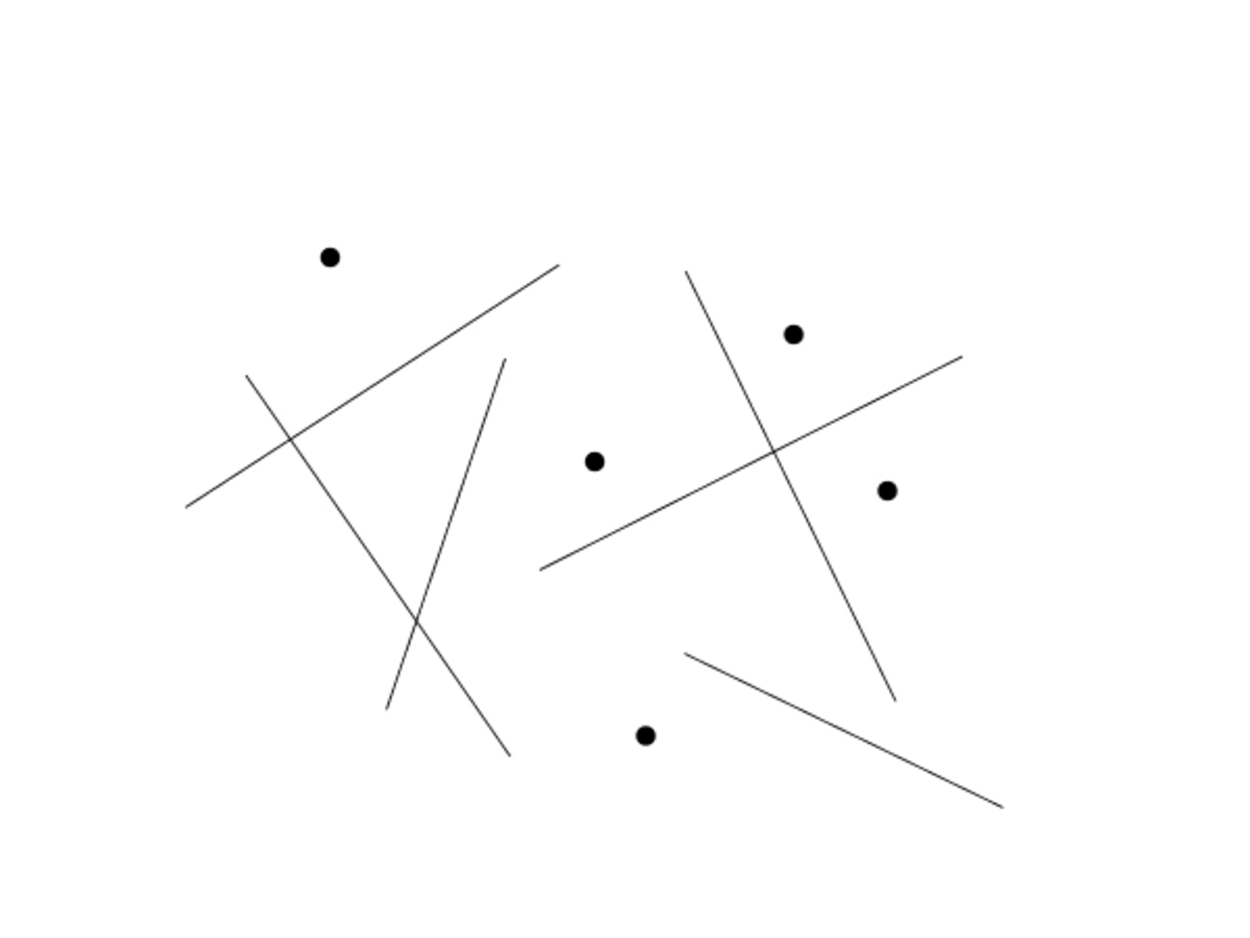
\includegraphics[width=60mm]{figure}\label{fig:subfigex_a}}\\
%\subfloat[][]{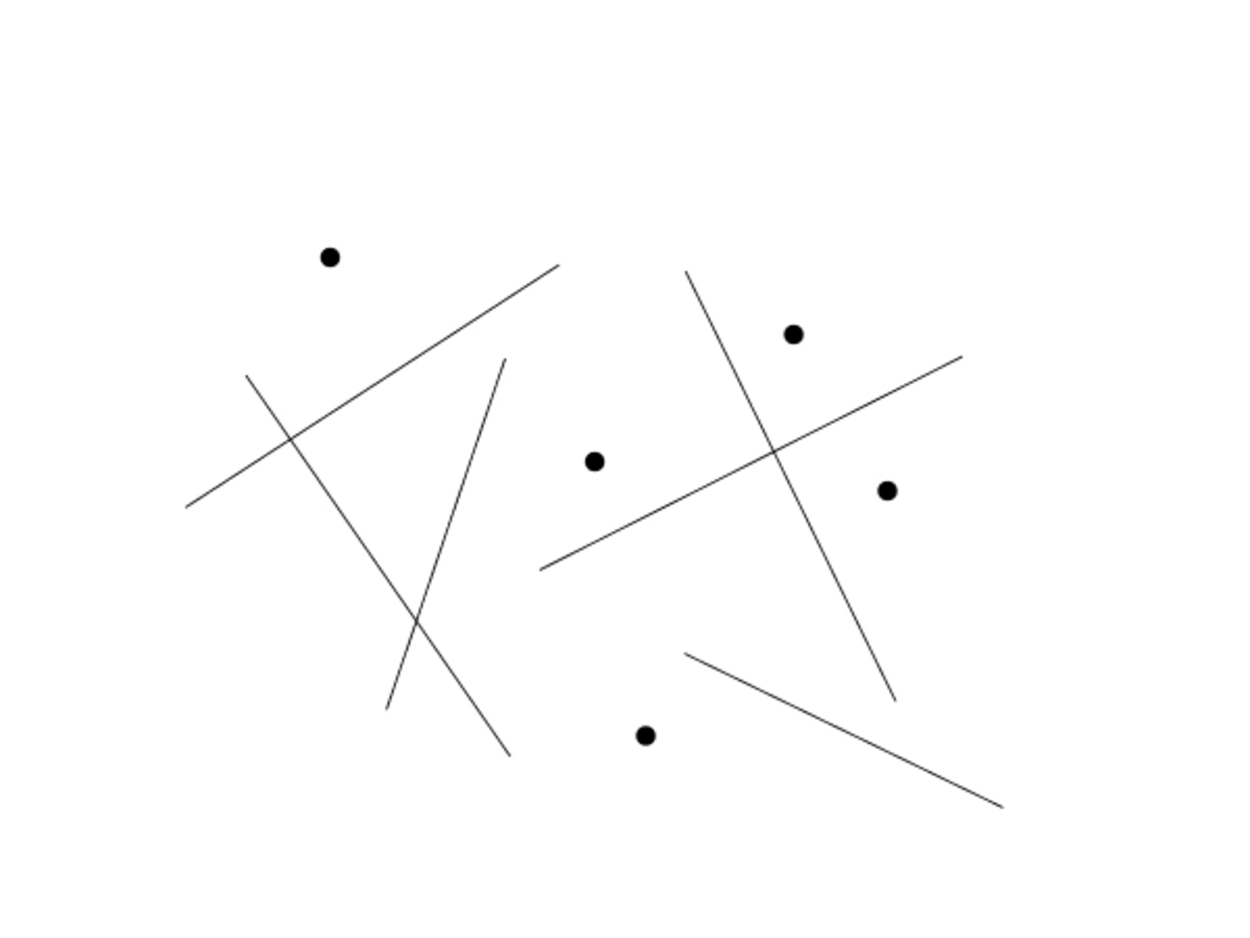
\includegraphics[width=80mm]{figure}\label{fig:subfigex_b}}
%}
%\caption{Here's an example using the subfig package.\label{fig:subfigex} }
%\end{figure}



\section{Citations}

All bibliographical references should be listed at the end, inside a numbered, first-level heading section titled REFERENCES.
References must be numbered in order of appearance. 
Reference numbers in the text should appear within square brackets, such as in~\cite{Someone:13} or~\cite{Someone:13,Someone:04,Someone:09}.
BibTeX will also handle this for you~\cite{ref:4,ref:online}.
Do not list references that do not appear in the text. 

Use references preferably for bibliographic items. Prefer footnotes to cite URLs.\footnote{My URL: http://tenor-conference.org/} 



\section{Conclusions}
To finish your full-length paper, end it with a conclusion; 
and after careful editing and a final spell-cheek,
submit it through the conference Submission System (see call for papers). 
\underline{Do not} send papers directly by e-mail.


\begin{acknowledgments}
At the end of the Conclusions, acknowledgements to people, projects, funding agencies, etc. can be included using the ``acknowledgments'' environment (similar to second-level heading, with no numbering).
\end{acknowledgments} 

%%%%%%%%%%%%%%%%%%%%%%%%%%%%%%%%%%%%%%%%%%%%%%%%%%%%%%%%%%%%%%%%%%%%%%%%%%%%%
%bibliography here
\balance % balance the columns on the last page

% use bibtex to generate the bibliography
\bibliography{tenor-template}

\end{document}
